
\hypertarget{menu_file}{}
\section{File}
\index{file menu}

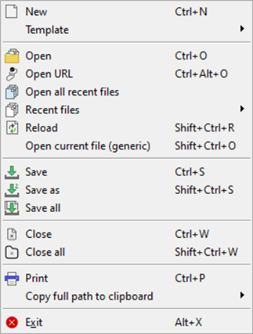
\includegraphics[scale=0.50]{./res/menu_file.png}\\

\begin{scriptsize}
  \begin{tabularx}{\textwidth}{>{\hsize=0.4\hsize}X>{\hsize=0.8\hsize}X}\\
    \hline
    \textbf{Option} & \textbf{Description} \\
    \hline
    New & Creates a new file \\
    Template & \textit{\href{\#menu\_file\_template}{See options ...}} \\
    Open & Opens selected file as text \\
    Open all recent files & Opens all files from the Most Recently Used (MRU) file list \\
    Recent files & Displays a Most Recently Used (MRU) file list. Selecting one of the displayed files will open that file \\
    Reload & Reloads the current files to the last saved status \\
    Save & Saves the current file. If the file has not been previously saved then the 'File Save As' dialog will open first \\
    Save as & Saves the current file with a new name \\
    Save all & Saves all changed files. If a file has not been previously saved the 'File Save As' dialog will open first \\
    Close & Closes the current file. If the file has not been saved you will be prompted to save it \\
    Close all & Closes all files including projects \\
    Print & Will open a Tinn-R dialog allowing settings and actions associated with the current file \\
    Copy full path to clipboard & \textit{\href{\#menu\_file\_copyfullpath}{See options ...}} \\
    Exit & Exits the application \\
    \hline
  \end{tabularx}
\end{scriptsize}

\hypertarget{menu_file_template}{}
\subsection{Template}
\index{file menu!template}
\index{template!R script}
\index{template!R html}
\index{template!R markdown}
\index{template!R noweb}
\index{template!LaTeX}

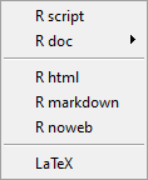
\includegraphics[scale=0.50]{./res/menu_file_template.png}\\

\begin{scriptsize}
  \begin{tabularx}{\textwidth}{>{\hsize=0.3\hsize}X>{\hsize=0.8\hsize}X}\\
    \hline
    \textbf{Option} & \textbf{Description} \\
    \hline
    R script & Creates a R script template \\
    R doc & \textit{\href{\#menu\_file\_template\_rdoc}{See options ...}} \\
    R html & Creates a R html template \\
    R markdown & Creates a R markdown template \\
    R noweb & Creates a R noweb template \\
    \LaTeX & Creates a \LaTeX ~template \\
    \hline
  \end{tabularx}
\end{scriptsize}


\newpage
\hypertarget{menu_file_template_rdoc}{}
\subsubsection{R doc}
\index{template!R doc}

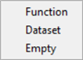
\includegraphics[scale=0.50]{./res/menu_file_template_rdoc.png}\\

\begin{scriptsize}
  \begin{tabularx}{\textwidth}{>{\hsize=0.3\hsize}X>{\hsize=0.8\hsize}X}\\
    \hline
    \textbf{Option} & \textbf{Description} \\
    \hline
    Function & Creates a R doc function template \\
    Dataset & Creates a R doc dataset template  \\
    Empty & Creates a R doc empty template \\
    \hline
  \end{tabularx}
\end{scriptsize}


\hypertarget{menu_file_copyfullpath}{}
\subsection{Copy full path to clipboard}
\index{file menu!copy to clipboard}

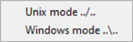
\includegraphics[scale=0.50]{./res/menu_file_copyfullpathtoclipboard.png}\\

\begin{scriptsize}
  \begin{tabularx}{\textwidth}{>{\hsize=0.3\hsize}X>{\hsize=0.8\hsize}X}\\
    \hline
    \textbf{Option} & \textbf{Description} \\
    \hline
    Unix mode ../.. & Copy full path of current file to clipboard in Unix mode ../.. \\
    Windows mode ..$\backslash$.. & Copy full path of current file to clipboard Windows mode ..$\backslash$.. \\
    \hline
  \end{tabularx}
\end{scriptsize}
